\chapter{Vorgehen}
Model der Machbarkeitsstudie ausmessen und Entwicklungspunkte definieren.

\section{Inbetriebnahme des Modells der Machbarkeitsstudie}
Mit der in der Projektarbeit entwickelten Harvesterschaltung kann per Bluetooth Smart auf dem Android-Endgerät die Geschwindigkeit ausgegeben werden.
Bei der Inbetriebnahme zeigten sich folgende Grenzen im gegebenen Modell:

\begin{enumerate}
    \item Zu hoher Kondensator vor Energiemanagmenetschaltung gefährdet deren Stabilität
    \item Konfiguration auf Energiemanagementboard sind nicht auf EnergieHarvesterSchaltung angepasst
    \item ???
\end{enumerate}



\subsubsection{Kapazität für Harvesting-Schaltung verbessern}
In der Machbarkeitsstudie ist nach dem Gleichrichter ein Kondensator von 470 uF nachgeschaltet. Dieser glättet die Spannungspulse nach dem Gleichrichter zu einer DC-ähnlichen Spannung mit Rippeln.

Mit einem Kondensator von 470 uF wird die Ausgangsspannung der Harvesterspannung fast rippelfrei.
\begin{figure}
\includegraphics[bb = 0 0 100 100]{3Vorgehen/imag/10uF.PNG}
\caption{Rippelspannung mit 10 uFKondensator}
\end{figure}

Was ideal aussieht ist für die nachfolgende Energiemanagmentschaltung nicht ideal. Für die 



Ives von EMMicroelectronics rät den Kondensator um den Faktor 10 zu verkleineren, da die nachfolgende Energiemanagementschaltung sonst nicht mit Sicherheit ordnungsgemäss funktioniert. 

Aus diesem Grund wird die Rippelspannung am Ausgangs der Harvesterschaltung mit kleineren Kondensatoren gemessen. Das Messprotokoll befindet sich im Anhang.

\subsubsection*{Messaufbau}

\begin{figure}
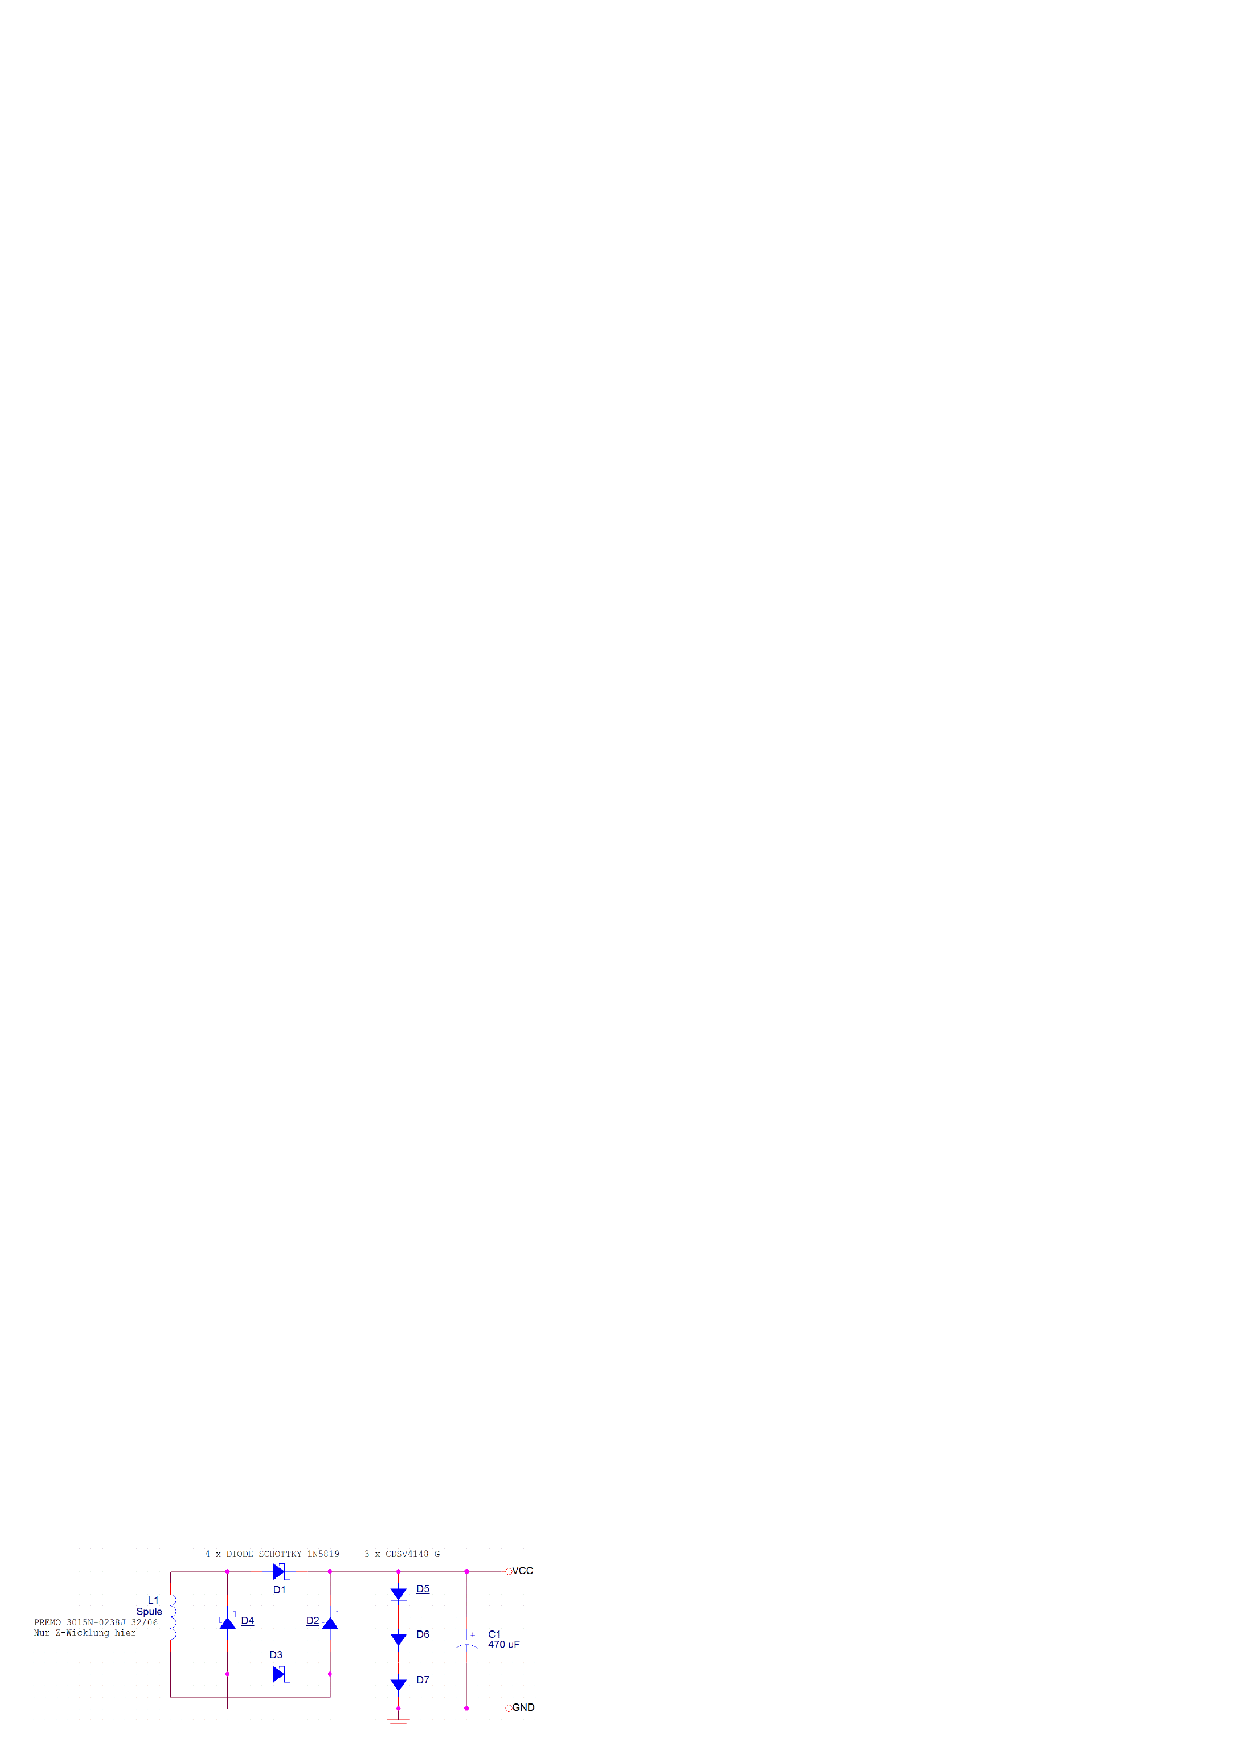
\includegraphics[bb = 0 0 100 100]{3Vorgehen/imag/messschaltungHarvesterschaltung.gif}
\caption{Messschaltung}
\end{figure}

\subsubsection*{Resultate}

\begin{figure}
\includegraphics[bb = 0 0 100 100]{3Vorgehen/imag/10uF.PNG}
\caption{Rippelspannung mit 10 uFKondensator}
\end{figure}

\begin{figure}
\includegraphics[bb = 0 0 100 100]{3Vorgehen/imag/47uF.PNG}
\caption{Rippelspannung mit 47 uFKondensator}
\end{figure}


\subsubsection{Messungen Energy Management Board}

\begin{figure}
\includegraphics[bb = 0 0 100 100]{3Vorgehen/imag/messungPA.png}
\caption{Rippelspannung mit 47 uFKondensator}
\end{figure}
Es zeigt sich, dass der LTS nicht geladen wird . Und es zeigt sich, dass das EM-Board nicht zu regulieren beginnt.








\pagebreak
\subsubsection{Messungen Sensortag}
Ziel: Energieverbrauch kennen.

Unterschied zwischen dem Programmierten Sensortag des Prototypen und dem neuen Sensortag.




\section{Layout Print}

\section{Kommunikation Bluetooth Low Energy}

\section{Energieoptimierung}



\section{Applikationsentwicklung}

\section{Option 1}






